\chapter{Fonctionnalités}
\label{s:fonctionnalite}

\section{Image}
\subsection{Importation}
Nom implémenté

\subsection{Exportation}
Implémenté

\subsection{Espace de couleur}
Implémenté

\subsection{Traitement d'image}
Implémenté

\subsection{Image procédurale}
Non implémenté

\section{Dessin vectoriel}
\subsection{Curseur dynamique}
Implémenté

\subsection{Primitives vectorielles}
Implémenté

\subsection{Formes vectorielles}
Implémenté

\subsection{Outils de dessin}
Implémenté

\subsection{Interface}
Implémenté

\section{Transformation}
\subsection{Transformation interactive}
Implémenté

\subsection{Structure de scène}
La structure de scène a été implémenté sous la forme d'un arbre ordoné, dans lequel les feuilles sont les éléments de la scène. La classe scène comprend 4 classes interne, soit element, group, node et scene\_iterator. Les classes group et node héritent d'element et  servent à stocker tout ce qui se trouve dans la scène. La classe scene\_iterator permet, quant-à elle, de parcourir les éléments pour les dessiner. 

On utilise les shared\_ptr au lieux des simples pointeurs pour conserver les éléments qui sont ajouté à la scène pour ne pas avoir à trop gérer la mémoire.

L'essentiel du code de la scène se trouve dans les méthodes addElement de la scène, des sous-clases de stockage et l'operator++ de l'itérateur.

\begin{lstlisting}
void scene::addElement(size_t index, primitive_ptr& p, bool insertFirstChild) {
	if (index == 0 && !insertFirstChild {
		throw invalid_argument("root don't have parent...");
	}
	root->addElement(index, p, insertFirstChild);
}

//Retourne la quantite d'element ajoute
size_t scene::node::addElement(size_t index, primitive_ptr& p, bool insertFirstChild) {
	if (index != this->index) {
		throw invalid_argument("index need to be equals to the index of the node");
	}
	if (insertFirstChild) {
		throw invalid_argument("node need to be wraped in a group");
	}
	this->content = p;
	contentType = "primitive";
	return 1;
}

//Retourne la quantite d'element ajoute
size_t scene::group::addElement(size_t index, primitive_ptr& p, bool insertFirstChild) {
	size_t addedSize = 0;
	
	if (this->index == index) {
		if (insertFirstChild) {
			//Inserer comme premier element
			childrens.insert(childrens.begin(), element_ptr{ new node{ index + 1, height + 1, p } });
			for (auto& it = childrens.begin() + 1; it < childrens.end(); ++it) {
				it->get()->setIndex(it->get()->getIndex() + 1);
			}
			addedSize++;
		} else {
			throw invalid_argument("element must to be add in the parent");
		}
	} else {
		size_t ubound = childrens.size();
		size_t lbound = 0;
		size_t i;
		
		//Recherche binaire
		while (lbound <= ubound) {
			i = lbound + (ubound - lbound) / 2;
			if (childrens[i]->getIndex() == index) {
				if (insertFirstChild) {
					if (childrens[i]->getType() != "group") {
						group_ptr temp = group_ptr{ new group{ index, height + 1 } };
						temp->childrens.push_back(childrens[i]);
						temp->childrens[0]->setIndex(index + 1);
						temp->childrens[0]->setHeight(height + 2);
						temp->size = temp->childrens[0]->getSize() + 1;
						childrens[i] = temp;
						addedSize++;
					}
					addedSize += childrens[i]->addElement(index, p, insertFirstChild);
				} else {
					childrens.insert(childrens.begin() + i + 1, element_ptr{ new node{ index + childrens[i]->getSize(), height + 1, p } });
					i++;
					addedSize++;
				}
				i++;
				break;
			} else if (childrens[i]->getIndex() < index) {
				lbound = i + 1;
				if (ubound < lbound) {
					//Ajoute l'element dans le groupe sous-jacent
					addedSize += childrens[i]->addElement(index, p, insertFirstChild);
					i++;
					break;
				}
			} else {
				ubound = i - 1;
				if (ubound < lbound) {
					//Ajoute l'element dans le groupe sous-jacent
					addedSize += childrens[i - 1]->addElement(index, p, insertFirstChild);
					break;
				}
			}
		}	
		for (auto& it = childrens.begin() + i; it < childrens.end(); ++it) {
			it->get()->setIndex(it->get()->getIndex() + addedSize);
		}
	}
	size += addedSize;
	return addedSize;
}

//Avance jusqu'au prochain node
void scene::scene_iterator::operator++() {
	for (rootIndex; rootIndex <= root->getSize(); ++rootIndex) {
		element* elem = root->getElement(rootIndex);
		if (elem->getType() != "group" && elem->getType() != "root") {
			primitive_ptr ptr = (dynamic_cast<node*>(elem))->content;
			if (p != ptr) {
				p = ptr;
				break;
			}
		}
	}
	if (rootIndex > root->getSize()) {
		p = primitive_ptr{ nullptr };
	}
}
\end{lstlisting}
Comme vous avez sans-doute remarqué, l'ajout d'élément à la scène se fait récursivement, à l'index en paramètre. Le paramètre «insertFirstChild» indique s'il faut insérer l'élément comme le premier enfant de l'élément à l'index en paramètre. S'il est faux, on insère simplement le nouvel élément après l'index. Dans group::addElement, on utilise un algorithme de recherche binaire pour trouver dans ou après quel élément il faut ajouter le nouvel élément.

L'operator++, quant à lui, parcours la scène en s'arrêtant seulement sur les classes node.  

Malheureusement, par manque de temps la structure de scène n'est pas utilisé à sont plein potentiel et tous les éléments sont stocké dans le groupe à la racine de la scène. Il est tout de même possible de voir le résultat en changeant la ligne «\#define test 0» pour «\#define test 1» dans le fichier «main.cpp». Vous verrez alors le résultat de l'exécution des tests de la classe scene (principalement de l'ajout et de la supression d'élément), se trouvant à la fin de «scene.cpp». 

\subsection{Sélection multiple}
Implémenté

\subsection{Coordonnées non-cartésiennes}
Non-implémenté

\subsection{Historique}
Non-implémenté

\section{Géométrie}
\subsection{Particules}
Non-implémenté

\subsection{Primitives}
Implémenté

\subsection{Modèle}
Implémenté

\subsection{Texture}
Implémenté

\subsection{Géométrie procédurale}
Non-implémenté

\pagebreak
\section{Caméra}
\subsection{Propriétés de caméra}
Helllo there????

\begin{figure}[h]
	\centering
	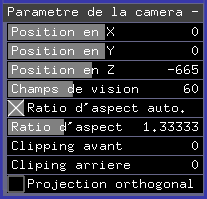
\includegraphics[width=5cm]{fig/proprieteCamera.png}
	\caption{Propriété de la caméra dans l'interface}
	\label{fig:test}
\end{figure}

\subsection{Mode de projection}
Le changement de mode de projection de perspective à orthogonale a été implémenté dans l'application. L'essentiel du travail se fait dans la méthode ccamera::changeMode(). Elle est appelé lorsqu'on appuit sur le bouton à cet effet dans l'interface graphique.

\begin{lstlisting}
	if (ortho.get()) {
		cam->enableOrtho();
	} else {
		cam->disableOrtho();
	}
\end{lstlisting}

\subsection{Caméra interactive}
La caméra interactive est implémenter dans l'application principalement à l'aide de la classe ofEasyCam de openFrameworks. Nous avons tout de même ajouter la possibilité de déplacer à l'aide des flèches du clavier, pour permettre de repositionner facilement la caméra. Il est aussi possible d'avancer à caméra à l'aide de pageUp/Down. L'essentiel du code se trouve au début de «ccamera::update()».

\begin{lstlisting}
	float dist = speed * dt;
	float dx = 0;
	float dy = 0;
	float dz = 0;
	
	dx = 0;
	if (isCameraMoveLeft)
		dx += dist;
	if (isCameraMoveRight)
		dx -= dist;
	cam->truck(-dx);
	posX.set(round(-cam->getX()));
	
	dy = 0;
	if (isCameraMoveUp)
		dy -= dist;
	if (isCameraMoveDown)
		dy += dist;
	cam->boom(-dy);
	posY.set(round(cam->getY()));
	
	dz = 0;
	if (isCameraMoveForward)
		dz -= dist;
	if (isCameraMoveBackward)
		dz += dist;
	cam->dolly(dz);
	posZ.set(round(cam->getZ()));
\end{lstlisting}

\subsection{Caméra multiple}
Non-implémenté

\subsection{Caméra animée}
Non-implémenté
